\subsection*{Timing}

\begin{figure}
\begin{centering}
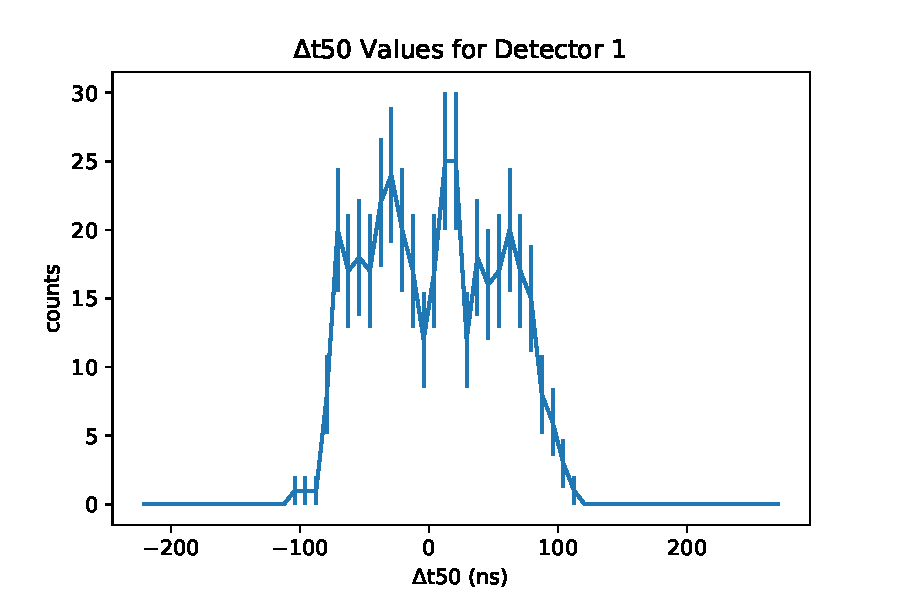
\includegraphics[width=0.7\textwidth]{./figures/t50s_det1.pdf}
\caption{The $\Delta t50$ distribution for detector 1.}
\label{t50_1}
\end{centering}
\end{figure}

Plotted is the distribution of $\Delta t50$ for both detectors. The source was located on the DC side of detector1. Events close to this face correspond to the most negative values of $\Delta t50$. We expect to see an exponential fall-off of events as depth increases from this point. There is some exponential trend, however, at the opposite side of the detector 

\begin{figure}
\begin{centering}
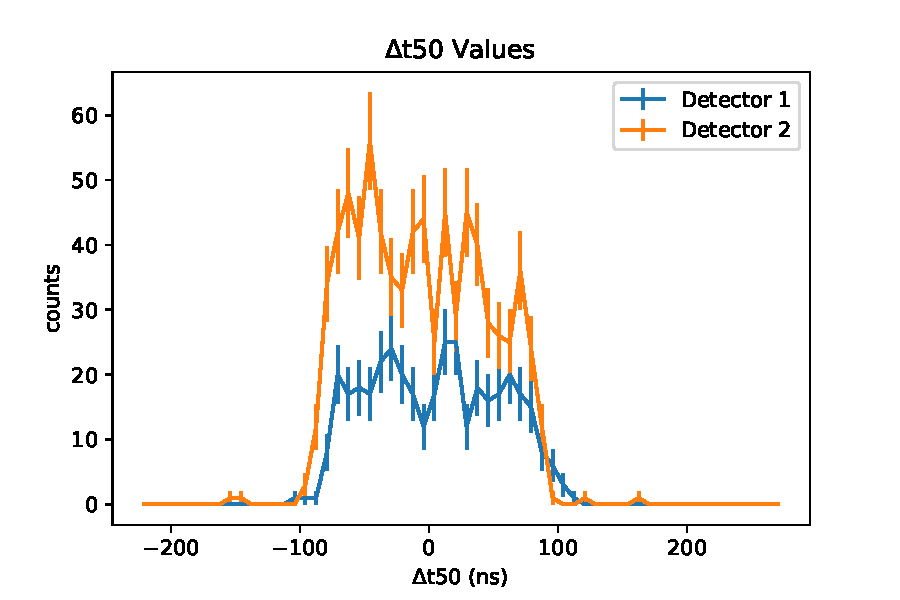
\includegraphics[width=0.7\textwidth]{./figures/t50s_det2.pdf}
\caption{The $\Delta t50$ distribution for detector 2.}
\label{t50_2}
\end{centering}
\end{figure}

The trigger time of a signal is determined by a on-board fast trapezoidal shaper. This trigger time may differ slightly between signals, depending on the location of the interaction, leading to additional uncertainty. The effect of this jitter will be studied for more precise position determination. Additionally, some events will be subject to charge sharing, charge loss in the inter-strip gap, collection to a disconnected strip, random coincidence, etc. All of these effects lead to errors in the $t50$ determination.

\subsection*{Depth Determination}

\begin{figure}
\begin{centering}
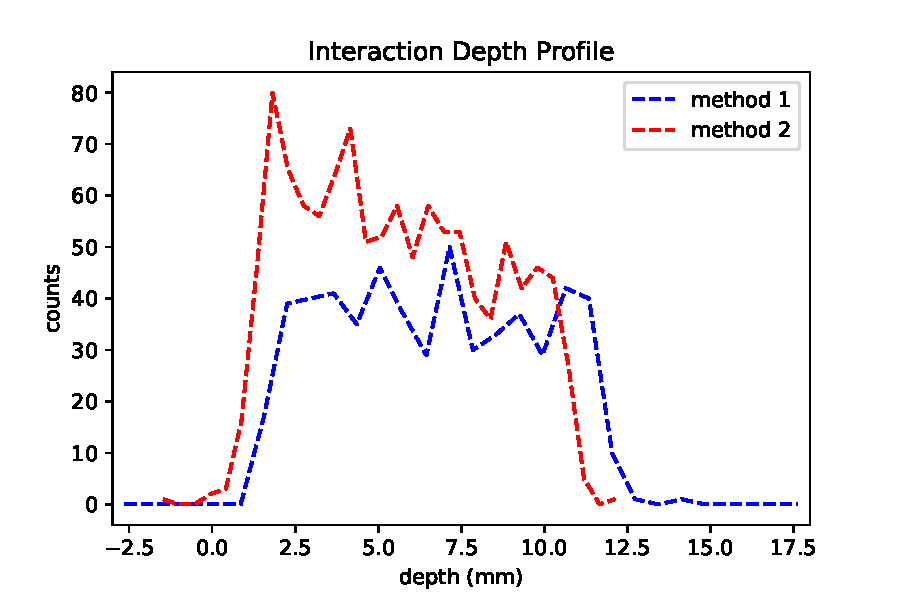
\includegraphics[width=0.7\textwidth]{./figures/interactiondepths.pdf}
\caption{The depths of interactions in detector 1 using two different methods of extracting depth from $\Delta t50$. Method 1 is a more simple linear fit, whereas method 2 takes into account the differences in charge carrier drift times.}
\label{depths}
\end{centering}
\end{figure}

The depth profile for detector 1 is shown in \ref{interactiondepths}. The second method of calculating depth, which takes into account the different carrier velocities, seems to give a better result. More events are confined within the detector and the depth profile looks to have a more apparent exponential trend.

Another source of error is scattering events. A gamma ray may scatter in an event with full-energy deposition (forward Compton scattering within a voxel for example), and the assumption of a single scattering event where there were two or more interactions will lead to an improperly reconstructed interaction position. This is another source of error in our measurement.

\subsection*{Comparison to Simulation}

A simple model was built in GEANT4 (two planar HPGe crystals, 74 mm wide, 15 mm thick, 10 mm apart). No surrounding material was included in the model. A point source emitting gamma-rays with energy 661.657 keV from a point 2 meters in front of the front-face of the first detector was used \cite{ebss}. This data was used to compare to the experimentally determined distribution of interaction depths. In \ref{g4} the z positions from single interactions in the single data are plotted alongside the reconstructed z positions from \ref{g4}. There is reasonable agreement between the two, although the reconstructed depths have an excess of events on the AC face of detector 1. Signals from events near the DC face are more likely to experience effects from charge trapping, due to poorer transport of holes. This could explain some of the discrepancy.

\begin{figure}
\begin{centering}
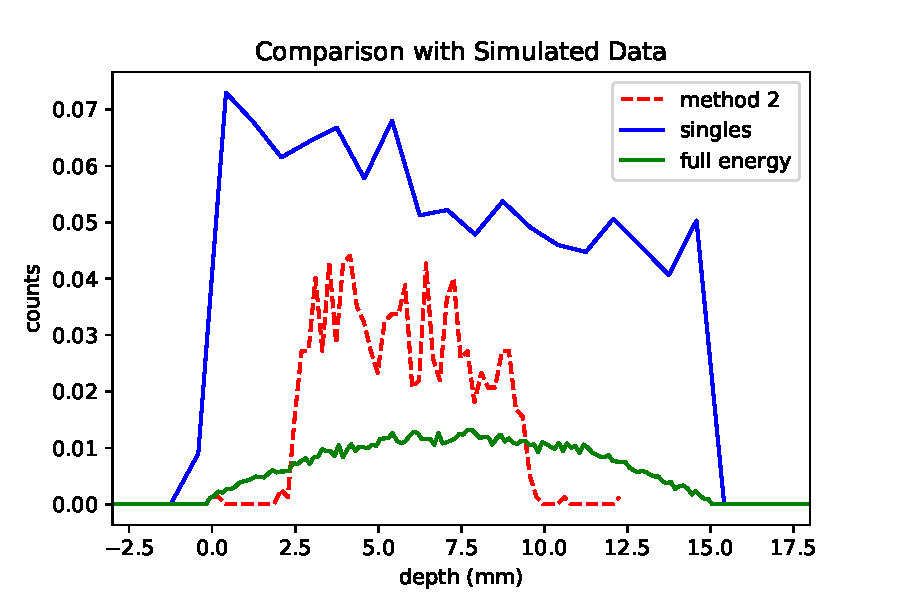
\includegraphics[width=0.7\textwidth]{./figures/g4_comp.pdf}
\caption{A comparison of simulated data (blue) and the reconstructed depths from experimental data (red). These data sets have been normalized. There is reasonable agreement between the two.}
\label{g4}
\end{centering}
\end{figure}

